% SUPERSEDED 12 Oct 2026: no longer input. Its content is condensed into lit_transport.tex (Section 2.1);
% fig:tension is not in the main text. Listed for deletion in docs/thesis_work_2026-10-12b.md.
% modelling.tex -- Literature review: cable models and their assumptions.
% Restructured 9 Oct (structure audit): the single-quadrotor model and fig:quad_frames are cut, the
% spring-damper equation is cut, and this thesis's own payload model moved to Source/src/model.tex
% (Methodology), merged with the planner's model. Simulation fidelity moved to Literature_review.tex.

\subsection{Cable-Suspended Transport and Model Assumptions}
\label{sec:lit_models}

The assumptions made about the cable set both the complexity of the dynamics and the validity of
the controller. The literature uses two models (Figure~\ref{fig:tension}).

\begin{figure}[h]
\centering
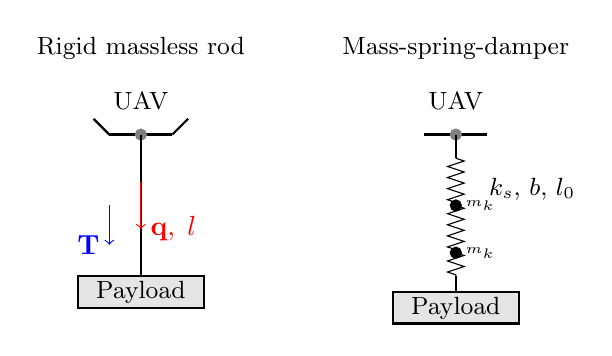
\begin{tikzpicture}[scale=1.0]
  % --- Left: Rigid rod ---
  \node[font=\small] at (-2, 3.5) {Rigid massless rod};

  % UAV
  \draw[thick] (-2.4,2.4) -- (-1.6,2.4);
  \draw[thick] (-2.4,2.4) -- (-2.6,2.6);
  \draw[thick] (-1.6,2.4) -- (-1.4,2.6);
  \filldraw[gray] (-2,2.4) circle (2pt);
  \node[above] at (-2,2.6) {\small UAV};

  % Rigid cable with unit vector label
  \draw[thick] (-2,2.4) -- (-2,0.6);
  \draw[->,red] (-2,1.8) -- (-2,1.2)
      node[right] {$\mathbf{q}, \; l$};

  % Payload
  \draw[thick,fill=gray!20] (-2.8,0.2) rectangle (-1.2,0.6);
  \node[font=\small] at (-2,0.4) {Payload};

  % Tension label
  \draw[->,blue] (-2.4,1.5) -- (-2.4,1.0)
      node[left] {$\mathbf{T}$};

  % --- Right: Spring-damper ---
  \node[font=\small] at (2, 3.5) {Mass-spring-damper};

  % UAV
  \draw[thick] (1.6,2.4) -- (2.4,2.4);
  \filldraw[gray] (2,2.4) circle (2pt);
  \node[above] at (2,2.6) {\small UAV};

  % Spring segments with lumped masses
  \draw[thick] (2,2.4) -- (2,2.1);
  \draw[decorate, decoration={zigzag,segment length=4pt, amplitude=3pt}]
      (2,2.1) -- (2,1.5);
  \filldraw (2,1.5) circle (2pt) node[right] {\tiny $m_k$};
  \draw[decorate, decoration={zigzag,segment length=4pt, amplitude=3pt}]
      (2,1.5) -- (2,0.9);
  \filldraw (2,0.9) circle (2pt) node[right] {\tiny $m_k$};
  \draw[decorate, decoration={zigzag,segment length=4pt, amplitude=3pt}]
      (2,0.9) -- (2,0.6);
  \draw[thick] (2,0.6) -- (2,0.4);

  % k_s and b labels
  \node[right, font=\small] at (2.3,1.7) {$k_s,\, b,\, l_0$};

  % Payload
  \draw[thick,fill=gray!20] (1.2,0.0) rectangle (2.8,0.4);
  \node[font=\small] at (2,0.2) {Payload};
\end{tikzpicture}
\caption{Cable modelling approaches.}
\label{fig:tension}
\end{figure}

The most common is the \textit{rigid massless rod}, adopted by \cite{efficient} and \cite{wahbaKinodynamicMotionPlanning2024}: a rigid link of fixed length $l$ along the unit vector $\mathbf{q}_i$, with the tension acting purely along it,

\begin{equation}
    \mathbf{T}_i = \lambda_i \mathbf{q}_i, \quad \lambda_i \geq 0
\end{equation}

where $\lambda_i$ is the tension, non-negative because a cable can pull but not push. The state stays compact and tractable, but slack cannot be captured.

The \textit{mass-spring-damper chain} of \cite{distributedNMPC} discretises the cable into $n$ lumped masses joined by spring--damper links of stiffness $k_s$, damping $b$ and rest length $l_0$. It captures sag and oscillation, at $6n$ extra states per cable.

Whatever the model, most controllers assume taut cables, with tension strictly positive throughout the task. A slack cable adds a unilateral constraint and a discontinuity in the equations of motion, and handling it rigorously remains open \cite{efficient}. For moderately aggressive indoor flight the rigid rod with taut cables is sufficient, consistent with \cite{tudelft}.
